\subsection{Qual é a precisão dos modelos na detecção de ambiguidade linguística em frases do Português Brasileiro?}\label{resultados-q-1}

Para avaliar a precisão dos modelos na detecção de ambiguidade seguimos a proposta de \cite{freitag2021funccao}, foram comparadas as acurácias e as matrizes de confusão obtidas, usando os dados da tarefa 1. Esta análise concentrou-se exclusivamente na detecção da presença ou ausência de ambiguidade, sem levar em consideração o tipo específico identificado pelos modelos posteriormente. Assim, os dados foram divididos em dois grupos distintos, totalizando 60 frases com ambiguidade e 60 frases distratoras. Foram realizadas duas coletas por frase, sendo obtidas 240 predições para cada modelo.


\begin{figure}[htb]
    \centering
    \begin{subfigure}[b]{0.45\textwidth}
        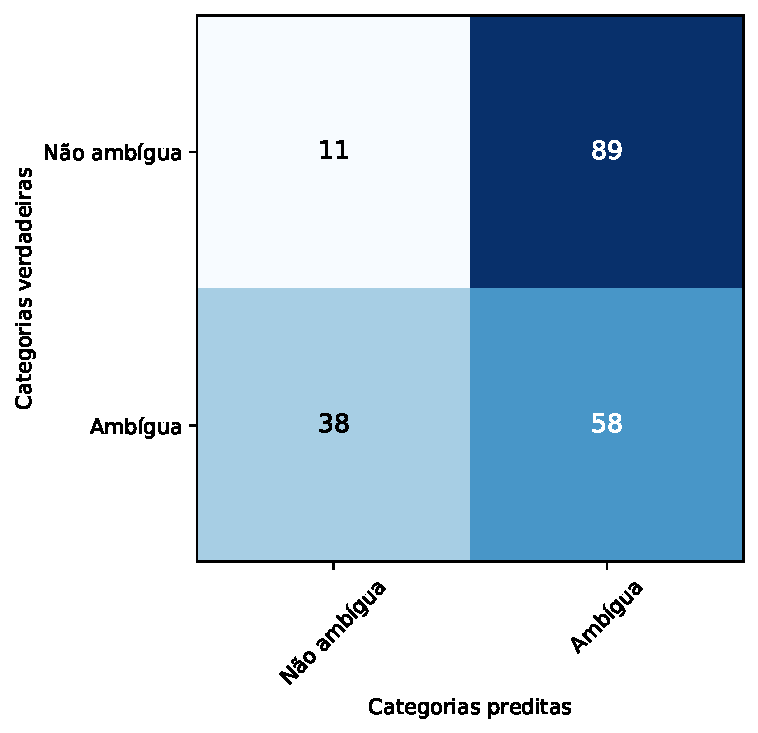
\includegraphics[width=\textwidth]{matriz_confusao_ChatGPT.pdf}
        \caption{Matriz de confusão do ChatGPT.}
        \label{fig:matriz_confusao_chatgpt}
    \end{subfigure}
    \hfill
    \begin{subfigure}[b]{0.45\textwidth}
        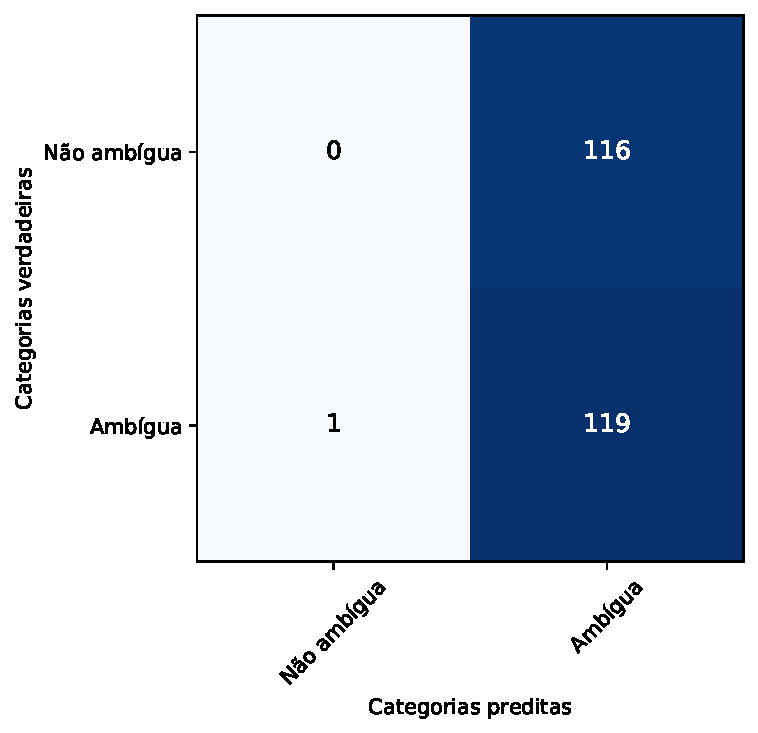
\includegraphics[width=\textwidth]{matriz_confusao_Bard.pdf}
        \caption{Matriz de confusão do Gemini.}
        \label{fig:matriz_confusao_bard}
    \end{subfigure}
    \caption{Matrizes de Confusão dos modelos ChatGPT e Gemini.}
    \label{fig:matriz_confusao_1}
\end{figure}

Os resultados da matriz de confusão na Figura \ref{fig:matriz_confusao_1} revelam que o ChatGPT registrou uma acurácia de apenas 28,75\%, enquanto o Gemini alcançou 49,58\%, indicando que estas versões dos modelos não conseguem detectar ambiguidade com precisão confiável. Os resultados revelam que ambos os modelos exibem uma quantidade significativa de falsos positivos, identificando ambiguidade em frases que carecem dela. Enquanto o ChatGPT demonstra erros distribuídos em todos os quadrantes da matriz, o Gemini tende a rotular quase todas as frases como ambíguas, resultando em uma taxa maior de falsos positivos. Para computar as matrizes de confusão e a acurácia foram consideradas apenas as respostas em que os modelos responderam \enquote{Sim} e \enquote{Não}, de modo que todas as respostas \enquote{Não Sei} foram descartadas. Assim, o ChatGPT destacou-se por apresentar mais dúvidas, conseguindo responder 196 perguntas enquanto o Gemini respondeu 236.


A diferença de acurácia entre os dois modelos pode ser atribuída ao fato do ChatGPT expressar dúvidas ao detectar frases ambíguas, declarando não saber ou negando a presença de ambiguidade. Analisando os três tipos de ambiguidade, observa-se que o ChatGPT lida melhor com ambiguidades semânticas e sintáticas, cometendo mais erros quando a ambiguidade é apenas lexical. Uma explicação é devida à estrutura da ambiguidade sintática ser descrita em estudos de processamento linguístico \cite{maiadimensoes} (1) e de processamento de linguagem natural \cite{padovani2022metodo}(2). Em contrapartida, o Gemini apresentou apenas um caso de falso negativo, acertando todos os outros testes em frases ambíguas. Entretanto, o Gemini tem a tendência de não distinguir entre frases ambíguas e não ambíguas, pois, em todos os testes, indica a presença de ambiguidade.


%\textbf{Sintática}.Dentre os 40 experimentos com ambiguidade feitos com o ChatGPT e Bard, a primeira inteligência constatou ambiguidade em 22 frases, mas por outro lado, o Gemini identificou integralmente as sentenças ambíguas ainda que nem todas estivessem com a classificação correta. No entanto, no experimento feito com as frases sem ambiguidade, o ChatGPT reconheceu alguma ambiguidade em 8 casos, alcançando uma acurácia final de 37,5\%, enquanto que o Gemini identificou ambiguidade em todos os testes, resultando, nessa etapa, 100\% de falsos positivos e chegando a uma acurácia de 50\%.  


